\subsection{Elektronik}
Der Aufbau der Elektronik des Edubot Modells ist relativ simpel gehalten und kann folgender schematischen Darstellung entnommen werden:

\begin{figure}[H]
  \centering
  \begin{minipage}[t]{14 cm}
  	\centering
  	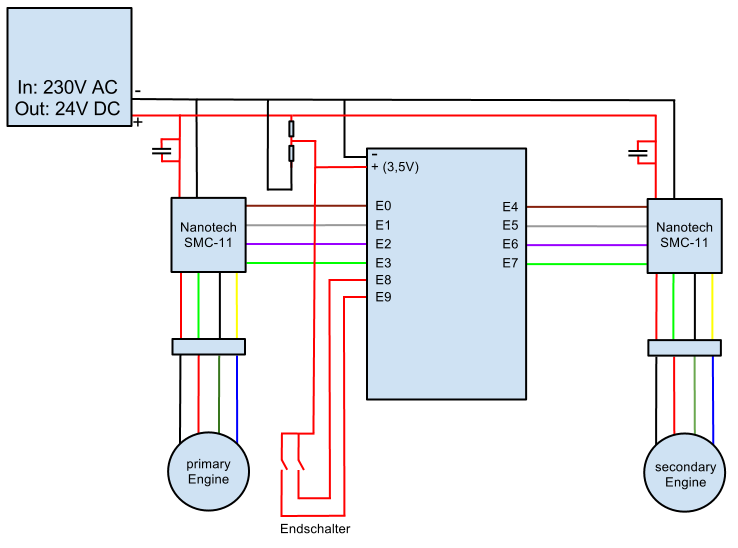
\includegraphics[width=14cm]{images/edubot_electronic} 
    \caption{Schematische Darstellung der Elektronik}
  \end{minipage}
\end{figure}

Bei der Erstellung der obigen Grafik wurde zu Gunsten der Übersichtlichkeit nicht darauf geachtet dass sich die Anschlüsse an den der Realität entsprechenden Seiten der Bauteile befinden, die Farbzuordnungen der Verbindungen entsprechen jedoch jenen der Tatsächlich verbauten Hardware.

\subsubsection{Motoren und Steuerungen}
Als Motoren kamen beim Edubot Modell zwei Schrittmotoren vom Typ ST2818 der Firma Nanotech zum Einsatz. Die beiden Motoren werden jeweils über eine separate Schrittmotorsteuerung gesteuert. Diese Schrittmotorteuerungen vom sind vom Typ Nanotech SMC-11 und übernehmen die Stromversorgung, sowie die direkte Ansteuerung der Motoren. Im Folgenden wird auf die einzelnen Bauteile noch etwas genauer eingegangen.

\begin{itemize}
\item \textbf{Steuerung}\\
Aufgabe der beiden Nanotech SMC-11 Steuerungen ist vor allem die direkte Ansteuerung der Motoren. Dazu muss sie über die 4 Verbindungskabel zum Motor Stromimpulse für das verfahren der einzelnen Takte übergeben.
Die beiden Motorsteuerungen verfügen jeweils über 4 Digitale Eingänge über die bestimmt wird wann der Motor einen Schritt fahren soll, in welche Richtung der Schritt gefahren werden soll, ob der Motor Ein- oder Ausgeschaltet ist und ob die Automatische Spannungsabsenkung (reduziert die Aufgenommene Leistung bei Stillstand des Motors nach 3 Sekunden automatisch um die Motorspulen zu schonen) aktiviert werden soll.
Die genannten Eingänge sind mit Ausgabepins des Mikrocontrollers verbunden. Damit übernimmt der Mikrocontroller die Übergabe der Parameter.

\item \textbf{Motoren}\\
Da es sich bei den beiden Motoren des Typs Nanotech ST2818 um bipolare Schrittmotoren handelt ermöglichen sie die Einteilung einer ganzen Umdrehung in eine bestimmte Anzahl an Schritten. Bipolar bedeutet das die Ansteuerung des Motors komplexer ist, dafür mehr Leistung abverlangt werden kann. Die Steuerung muss hierzu den bipolaren Betrieb eines Motors unterstützen.
In diesem Projekt wurde der 16 fache Mikroschrittmodus gewählt. Dieser ermöglicht die Teilung der einzelnen Schritte des Motors in 16 Teilschritte um damit eine höhere Genauigkeit zu erreichen. Der Spezifikation der Motoren ist zu entnehmen, dass ein Vollschritt 1,8$^\circ$ hat, ein Mikroschritt wie er beim Edubot Modell verwendet wird sind also 0,1125$^\circ$. 

\item \textbf{Endschalter}\\
Um den Roboter in seine Ausgangsposition fahren zu können, muss er zuerst an die Grenzen seines Arbeitsbereichs fahren. Von dort aus weiß der Mikrocontroller welche Winkel die einzelnen Motoren fahren müssen um in die Ausgangsposition zu kommen.
Damit erkannt werden kann wann die Grenzen des Arbeitsbereichs erreicht sind, wurden zwei Endschalter in Form von einfachen Kontaktstellen an den beiden Achsen und an der Basis angebracht. Stößt der Arm nun im Rahmen des "'Homings"' (Finden der Ausgangsposition) an die Basis, bzw. erreicht die sekundäre Achse ihren Maximalwinkel, so wird ein Kontakt hergestellt und der Mikrocontroller empfängt an einem Digitalen Eingang ein Signal. Realisiert wurden die Kontaktstellen als einfache Flächen aus Stahl, wobei auf die Verwendung vorgefertigter mechanischer Endschalter bewusst verzichtet wurde um Probleme mit dem Druckpunkt zu vermeiden. Nähere Informationen zum Ablauf des "'Homings"' finden sich im Unterkapitel "'Der Homing Algorithmus"' des Kapitels "'Der Mikrocontroller"'.
\end{itemize}


